\documentclass{article}
\usepackage{assignment_preamble}

\title{Lab 4}
\author{Ravi Kini}
\date{November 30, 2023}

\begin{document}

\maketitle

\repository{https://github.com/ravidosa/notes/tree/main/academics/assignments/code/phy112l_lab4}

\problem
For a given microstate and some site in the Ising model, we note that the microstate obtained by switching the spin of every site has an energy equal in both magnitude as sign, as every alignment remains the same. Further, this microstate is unique, as if two microstates have the same corresponding microstate, applying the switching transformation should yield the original microstate, which implies that the two microstates are the same. Consequently, every microstate has a unique corresponding microstate with equal energy and opposite spin for the specified site. For a given temperature, all the microstates with a certain energy will be accessible, and by pairing the corresponding microstates when summing the energies of every accessible microstate, we see that since the spins are opposite and the probability of the microstates are equal due to the energy being equal, the expected value of the spin is zero, so $\langle S_n \rangle = 0$ for all $n \in \{0, \ldots, 9\}$. 

\clearpage

\problem

For a quantity $x$ that takes value $x = 2$ with probability $p = 0.3$ or $x = 7$ with probability $p = 0.7$ and a quantity $y$ that takes value $y = 1$ with probability $p = 0.5$, $y = 3$ with probability $p = 0.4$, or $y = 4$ with probability $p = 0.1$,  the quantities have expected values of:
\begin{equation}
    \begin{split}
        \langle x \rangle & = 2\left(0.3\right) + 5\left(0.7\right) = 4.1 \\
        \langle y \rangle & = 1\left(0.5\right) + 3\left(0.4\right) + 4\left(0.1\right) = 2.1 \\
    \end{split}
\end{equation}

\begin{center}
\begin{tabular}{|c|c|c|}
    \hline
    $\left(x, y\right)$ & $xy$ & $p$  \\
    \hline
    $\left(2, 1\right)$ & $2 \cdot 1 = 2$ & $\left(0.3\right)\left(0.5\right) = 0.15$ \\
    \hline
    $\left(2, 3\right)$ & $2 \cdot 3 = 6$ & $\left(0.3\right)\left(0.4\right) = 0.12$ \\
    \hline
    $\left(2, 4\right)$ & $2 \cdot 4 = 8$ & $\left(0.3\right)\left(0.1\right) = 0.03$ \\
    \hline
    $\left(5, 1\right)$ & $5 \cdot 1 = 5$ & $\left(0.7\right)\left(0.5\right) = 0.35$ \\
    \hline
    $\left(5, 3\right)$ & $5 \cdot 3 = 15$ & $\left(0.7\right)\left(0.4\right) = 0.28$ \\
    \hline
    $\left(5, 4\right)$ & $5 \cdot 4 = 20$ & $\left(0.7\right)\left(0.1\right) = 0.07$ \\
    \hline
\end{tabular}
\end{center}
The probabilities sum to 1, as expected.

\begin{equation}
    \begin{split}
        \langle xy \rangle & = 2\left(0.15\right) + 6\left(0.12\right) + 8\left(0.03\right) + 5\left(0.35\right) + 15\left(0.28\right) + 20\left(0.07\right) = 8.61 \\
    \end{split}
\end{equation}
The correlation function is then:
\begin{equation}
    \begin{split}
        C\left(x, y\right) & = \langle xy \rangle - \langle x \rangle \langle y \rangle \\
        & = 8.61 - \left(4.1\right)\left(2.1\right) = 0
    \end{split}
\end{equation}
This result is reasonable, as the probabilities of $x$ and $y$ are independent and should show no correlation.

\clearpage

\problem
Since $\langle S_n \rangle = 0$ for all $n \in \{0, \ldots, 9\}$,  $\langle S_0\rangle, \langle S_r \rangle = 0$, so $C(S_0, S_r) = \langle S_0S_r \rangle - \langle S_0\rangle\langle S_r \rangle = \langle S_0S_r \rangle$.

\clearpage

\problem
The spin-spin correlation decreases as $r$ increases, with the rate of decrease being faster as $T$ increases. The program outputs:
    \begin{center}
    \begin{tabular}{|c|c|c|c|c|} \hline 
\multicolumn{2}{|c|}{\multirow{2}{*}{$C(r) = \langle S_0 S_r \rangle$}} &                                                   
  \multicolumn{3}{|c|}{$T$ }  \\ \cline{3-5} 
\multicolumn{2}{|c|}{}   & $0.5$ & $1.0$ & $1.5$ \\ \cline{1-5} 
\multirow{3}{*}{$r$} 
& $0$ & $1.000$ & $1.000$ & $1.000$ \\ \cline{2-5} 
& $1$ & $0.964$ & $0.762$ & $0.583$ \\ \cline{2-5} 
& $2$ & $0.929$ & $0.580$ & $0.340$ \\ \cline{2-5} 
& $3$ & $0.896$ & $0.442$ & $0.198$ \\ \cline{2-5} 
& $4$ & $0.864$ & $0.446$ & $0.115$ \\ \cline{2-5} 
& $5$ & $0.833$ & $0.256$ & $0.067$ \\ \cline{2-5} 
& $6$ & $0.803$ & $0.195$ & $0.039$ \\ \cline{2-5} 
& $7$ & $0.774$ & $0.149$ & $0.023$ \\ \cline{2-5} 
& $8$ & $0.746$ & $0.113$ & $0.013$ \\ \cline{2-5} 
& $9$ & $0.719$ & $0.086$ & $0.008$ \\ \hline 
\end{tabular}
    \end{center}

\clearpage

\problem
Figure \ref{fig:fig1} is a plot of $\ln C\left(r\right)$ vs. $r$ for $J = 1$ and $N = 10$. The plot is linear with negative slope and a y-intercept of $0$ which indicates that $\ln C\left(r\right) = -mr$ for some $m$. Consequently, $C\left(r\right) = e^{-mr} = e^{-\frac{r}{\xi}}$ for correlation length $\xi = \frac{1}{m}$.

\begin{figure}[!htb]
    \centering
    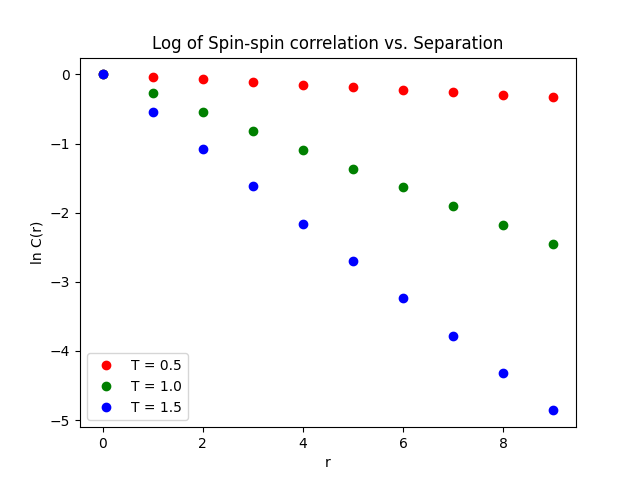
\includegraphics[width=0.75\textwidth]{../code/phy112l_lab4/4-5.png}
    \caption{Plot of log of spin-spin correlation against separation ($J = 1, N = 10$).}
    \label{fig:fig1}
\end{figure}

\clearpage

\problem
The correlation length $\xi$ can be estimated from the simulation by taking the average of $-\frac{r}{\ln C\left(r\right)}$ for values of separation $r$ for a given temperature $T$. We see that $\xi \approx {\left(-\ln\tanh\frac{J}{T}\right)}^{-1}$.
\begin{center}
    \begin{tabular}{|c|c|c|}
        \hline
        $\xi = \frac{1}{9}\sum_{r=1}^{9} -\frac{r}{\ln C(r)}$ & $-\ln\tanh\frac{J}{T}$ & ${\left(-\ln\tanh\frac{J}{T}\right)}^{-1}$ \\
        \hline
        $27.296022136$ & 
        $0.036635374$ &
        $27.296022137$\\
        \hline
        $3.6718609325$ & 
        $0.2723414689$ & 
        $3.6718609325$ \\
        \hline
        $1.8520560293$ & 
        $0.5399404683$ & 
        $1.8520560294$ \\
        \hline
    \end{tabular}
\end{center}

\clearpage

\problem
Figure \ref{fig:fig2} is a plot of $\langle E \rangle, C, S, F$ vs. $T$ for $J = 1$ and $N = 4 \times 4$. As $T$ increases, the average energy and entropy increase, while the free energy decreases. The specific heat peaks at a certain point, then decreases with increasing temperature.
\begin{figure}[!htb]
    \centering
    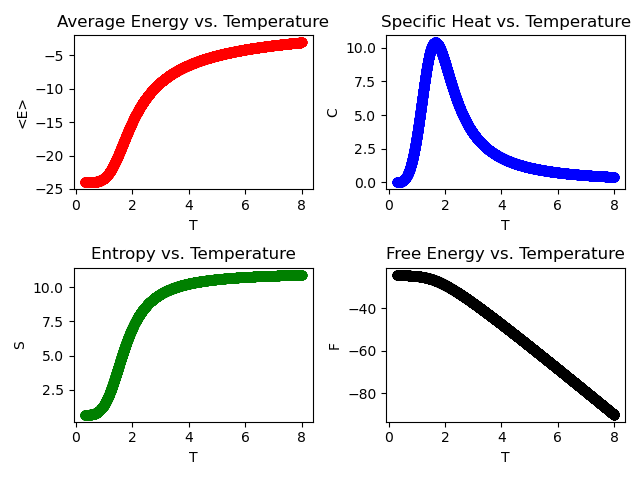
\includegraphics[width=0.75\textwidth]{../code/phy112l_lab4/4-7.png}
    \caption{Plot of average energy, specific heat, entropy, and free energy vs. temperature ($J = 1, N = 4 \times 4$).}
    \label{fig:fig2}
\end{figure}

\end{document}